\section{Methodology}

\subsection{Principal Component Analysis}

% https://www.aanda.org/articles/aa/full_html/2025/11/aa53461-24/aa53461-24.html

\begin{figure}[h!]
    \centering
    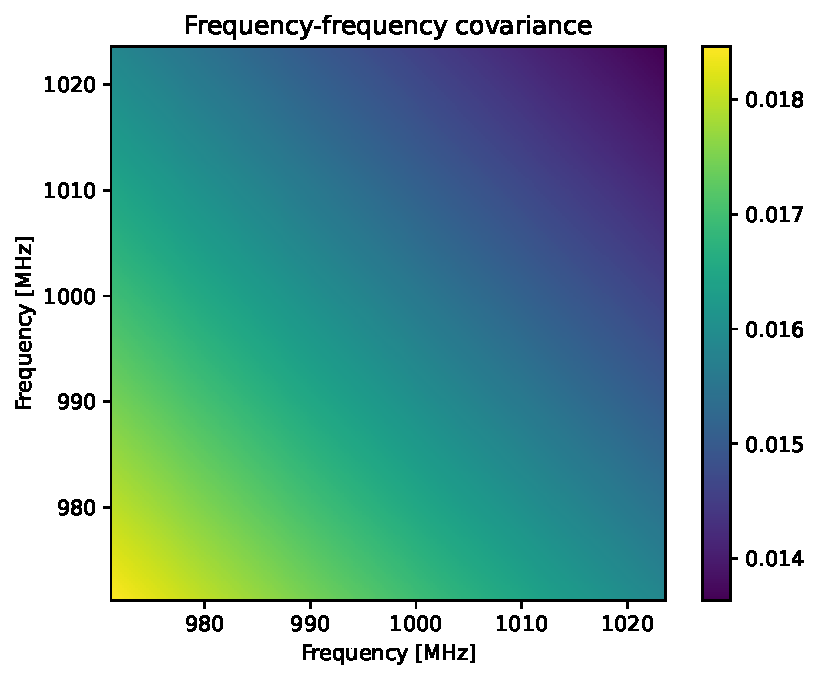
\includegraphics[width=1\linewidth]{outputs/week3/frequency_frequency_covariance.pdf}
    \caption{Frequency-frequency covariance matrix which is dominated by the foregrounds.}
    \label{fig:freq_covariance}
\end{figure}

\begin{figure}[h!]
    \centering
    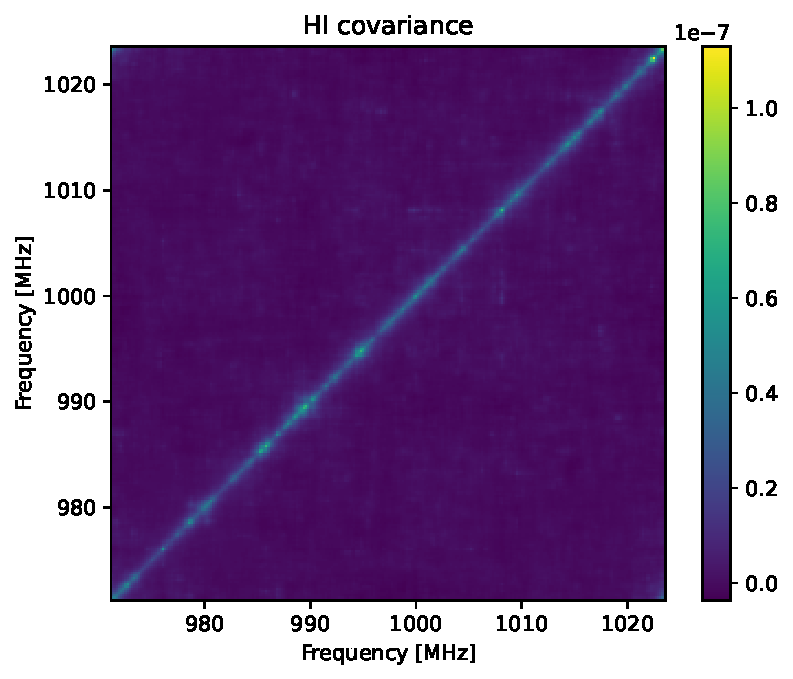
\includegraphics[width=1\linewidth]{outputs//week3/HI_covariance.pdf}
    \caption{HI covariance signal which is plotted separately from the foregrounds.}
    \label{fig:HI_covariance}
\end{figure}


By generating mock data using meer21cm, the frequency-frequency covariance can be plotted for the total signal of the 21cm signal and the foregrounds, seen in \cref{fig:freq_covariance}. We can see this is dominated by the foregrounds. The HI signal plotted separately can be seen in \cref{fig:HI_covariance}.

% provide more information on what kperp and kpara represents
From this HI map, the power spectrum was extracted. This power spectrum is a function of $k_\perp$ and $k_\parallel$ and provides information on how matter is distributed in the Universe. This can be seen in \cref{fig:power_spectrum_from_hydrogen_map}. The mock data can be generated using a fixed seed for random number generation, producing a specific outcome of a stochastic model known as a realisation. By running multiple realisations, the many different but equally likely outcomes of the mock data can be generated and used to quantify uncertainty. This was done by passing in various seed numbers to obtain uncertainties on the mock data. By averaging the power spectra into a 1D spectrum, the mock data can be compared to the input theory data. 

\subsection{Gaussian Process Regression}